\documentclass[a4paper,10pt]{article}
\usepackage[american]{babel} % for correct language and hyphenation and stuff
\usepackage[none]{hyphenat}
\usepackage{calc}            % for easier length calculations (infix notation)
\usepackage{enumitem}        % for configuring list environments
\usepackage{fancyhdr}        % for setting header and footer
\usepackage{fontspec}        % for fonts
\usepackage{geometry}        % for setting margins (\newgeometry)
\usepackage{graphicx}        % for pictures
\usepackage{microtype}       % for micro typography stuff
\usepackage{xcolor}          % for colours
\usepackage{lastpage}
\usepackage{fancyhdr}
\fancyhead{}
\fancyfoot{}
\rfoot{\thepage{}~of~\pageref{LastPage}}
\pagestyle{fancy}
\renewcommand{\headrulewidth}{0pt}
\renewcommand{\footrulewidth}{0pt}

% margins
\newgeometry{left=15mm,right=15mm,top=15mm,bottom=15mm}
% width of the gap between left and right column
\newlength{\cvcolumngapwidth}
\setlength{\cvcolumngapwidth}{2mm}
% left column width
\newlength{\cvleftcolumnwidth}
\setlength{\cvleftcolumnwidth}{38mm}
% right column width
\newlength{\cvrightcolumnwidth}
\setlength{\cvrightcolumnwidth}{\textwidth-\cvleftcolumnwidth-\cvcolumngapwidth}
% set paragraph indentation to 0
\setlength{\parindent}{0mm}


% style definitions
% style categories explanation:
% * \cvnameXXX is used for the name;
% * \cvsectionXXX is used for section names (left column, accompanied by a horizontal rule);
% * \cvtitleXXX is used for job/education titles (right column);
% * \cvdurationXXX is used for job/education duration (left column);
% * \cvheadingXXX is used for headings (left column);
% * \cvmainXXX (and \setmainfont) is used for main text;
% * \cvruleXXX is used for the horizontal rules denoting sections.

% font families
\defaultfontfeatures{Ligatures=TeX} % reportedly a good idea, see https://tex.stackexchange.com/a/37251
\newfontfamily{\cvnamefont}{Ubuntu Medium}
\newfontfamily{\cvsectionfont}{Ubuntu Medium}
\newfontfamily{\cvtitlefont}{Ubuntu} % Regular
\newfontfamily{\cvdurationfont}{Ubuntu Light Italic}
\newfontfamily{\cvheadingfont}{Ubuntu} % Regular
\setmainfont{Ubuntu Light}

% \defaultfontfeatures{Ligatures=TeX} % reportedly a good idea, see https://tex.stackexchange.com/a/37251
% \newfontfamily{\cvnamefont}{Roboto Medium}
% \newfontfamily{\cvsectionfont}{Roboto Medium}
% \newfontfamily{\cvtitlefont}{Roboto Regular}
% \newfontfamily{\cvdurationfont}{Roboto Light Italic}
% \newfontfamily{\cvheadingfont}{Roboto Regular}
% \setmainfont{Roboto Light}

% colours
\definecolor{cvnamecolor}{rgb}{0.2,0.2,0.2}
\definecolor{cvsectioncolor}{rgb}{0.2,0.2,0.2}
\definecolor{cvtitlecolor}{rgb}{0,0,0}
\definecolor{cvdurationcolor}{rgb}{0,0,0}
\definecolor{cvheadingcolor}{rgb}{0,0,0}
\definecolor{cvmaincolor}{rgb}{0,0,0}
\definecolor{cvrulecolor}{rgb}{0.2,0.2,0.2}
\color{cvmaincolor}

% styles
\newcommand{\cvnamestyle}[1]{{\Large\cvnamefont\textcolor{cvnamecolor}{#1}}}
\newcommand{\cvsectionstyle}[1]{{\normalsize\cvsectionfont\textcolor{cvsectioncolor}{#1}}}
\newcommand{\cvtitlestyle}[1]{{\normalsize\cvtitlefont\textcolor{cvtitlecolor}{#1}}}
\newcommand{\cvdurationstyle}[1]{{\normalsize\cvdurationfont\textcolor{cvdurationcolor}{#1}}}
\newcommand{\cvheadingstyle}[1]{{\normalsize\cvheadingfont\textcolor{cvheadingcolor}{#1}}}

% inter-item spacing
% vertical space after personal info and standard CV items
\newlength{\cvafteritemskipamount}
\setlength{\cvafteritemskipamount}{5mm plus 1.25mm minus 1.25mm}
% vertical space after sections
\newlength{\cvaftersectionskipamount}
\setlength{\cvaftersectionskipamount}{2mm plus 0.5mm minus 0.5mm}
% extra vertical space to be used when a section starts with an item with a heading (e.g. in the skills section), so that the heading does not follow the section name too closely
\newlength{\cvbetweensectionandheadingextraskipamount}
\setlength{\cvbetweensectionandheadingextraskipamount}{1mm plus 0.25mm minus 0.25mm}

% intra-item spacing
% vertical space after name
\newlength{\cvafternameskipamount}
\setlength{\cvafternameskipamount}{3mm plus 0.75mm minus 0.75mm}
% vertical space after personal info lines
\newlength{\cvafterpersonalinfolineskipamount}
\setlength{\cvafterpersonalinfolineskipamount}{2mm plus 0.5mm minus 0.5mm}
% vertical space after titles
\newlength{\cvaftertitleskipamount}
\setlength{\cvaftertitleskipamount}{1mm plus 0.25mm minus 0.25mm}
% value to be used as parskip in right column of CV items and itemsep in lists (same for both, for consistency)
\newlength{\cvparskip}
\setlength{\cvparskip}{0.5mm plus 0.125mm minus 0.125mm}
% set global list configuration (use parskip as itemsep, and no separation otherwise)
\setlist{parsep=0mm,topsep=0mm,partopsep=0mm,itemsep=\cvparskip}

% CV commands
% creates a "personal info" CV item with the given left and right column contents, with appropriate vertical space after
% @param #1 left column content (should be the CV photo)
% @param #2 right column content (should be the name and personal info)

\newcommand{\cvpersonalinfo}[2]{
    % left and right column
    \begin{minipage}[t]{\cvleftcolumnwidth}
        \vspace{0mm} % XXX hack to align to top, see https://tex.stackexchange.com/a/11632
        \raggedleft #1
    \end{minipage}% XXX necessary comment to avoid unwanted space
    \hspace{\cvcolumngapwidth}% XXX necessary comment to avoid unwanted space
    \begin{minipage}[t]{\cvrightcolumnwidth}
        \vspace{0mm} % XXX hack to align to top, see https://tex.stackexchange.com/a/11632
        #2
    \end{minipage}
    % space after
    \vspace{\cvafteritemskipamount}}

% typesets a name, with appropriate vertical space after
% @param #1 name text
\newcommand{\cvname}[1]{
    % name
    \cvnamestyle{#1}
    % space after
    \vspace{\cvafternameskipamount}}

% typesets a line of personal info beginning with an icon, with appropriate vertical space after
% @param #1 parameters for the \includegraphics command used to include the icon
% @param #2 icon filename
% @param #3 line text
\newcommand{\cvpersonalinfolinewithicon}[3]{
    % icon, vertically aligned with text (see https://tex.stackexchange.com/a/129463)
    \raisebox{.5\fontcharht\font`E-.5\height}{\includegraphics[#1]{#2}}
    % text
    #3
    % space after
    \vspace{\cvafterpersonalinfolineskipamount}}

% creates a "section" CV item with the given left column content, a horizontal rule in the right column, and with appropriate vertical space after
% @param #1 left column content (should be the section name)
\newcommand{\cvsection}[1]{
    % left and right column
    \begin{minipage}[t]{\cvleftcolumnwidth}
        \raggedleft\cvsectionstyle{#1}
    \end{minipage}% XXX necessary comment to avoid unwanted space
    \hspace{\cvcolumngapwidth}% XXX necessary comment to avoid unwanted space
    \begin{minipage}[t]{\cvrightcolumnwidth}
        \textcolor{cvrulecolor}{\rule{\cvrightcolumnwidth}{0.5mm}}
    \end{minipage}
    % space after
    \vspace{\cvaftersectionskipamount}}

% creates a standard, multi-purpose CV item with the given left and right column contents, parskip set to cvparskip in the right column, and with appropriate vertical space after
% @param #1 left column content
% @param #2 right column content
\newcommand{\cvitem}[2]{
    % left and right column
    \begin{minipage}[t]{\cvleftcolumnwidth}
        \raggedleft #1
    \end{minipage}% XXX necessary comment to avoid unwanted space
    \hspace{\cvcolumngapwidth}% XXX necessary comment to avoid unwanted space
    \begin{minipage}[t]{\cvrightcolumnwidth}
        \setlength{\parskip}{\cvparskip} #2
    \end{minipage}
    % space after
    \vspace{\cvafteritemskipamount}}

% typesets a title, with appropriate vertical space after
% @param #1 title text
\newcommand{\cvtitle}[1]{
    % title
    \cvtitlestyle{#1}
    % space after
    \vspace{\cvaftertitleskipamount}
    % XXX need to subtract cvparskip here, because it is automatically inserted after the title "paragraph"
    \vspace{-\cvparskip}}


% header and footer
% set "current page number of total page number"
\thispagestyle{fancy}

% preamble end/document start
\begin{document}

% personal info
\cvpersonalinfo{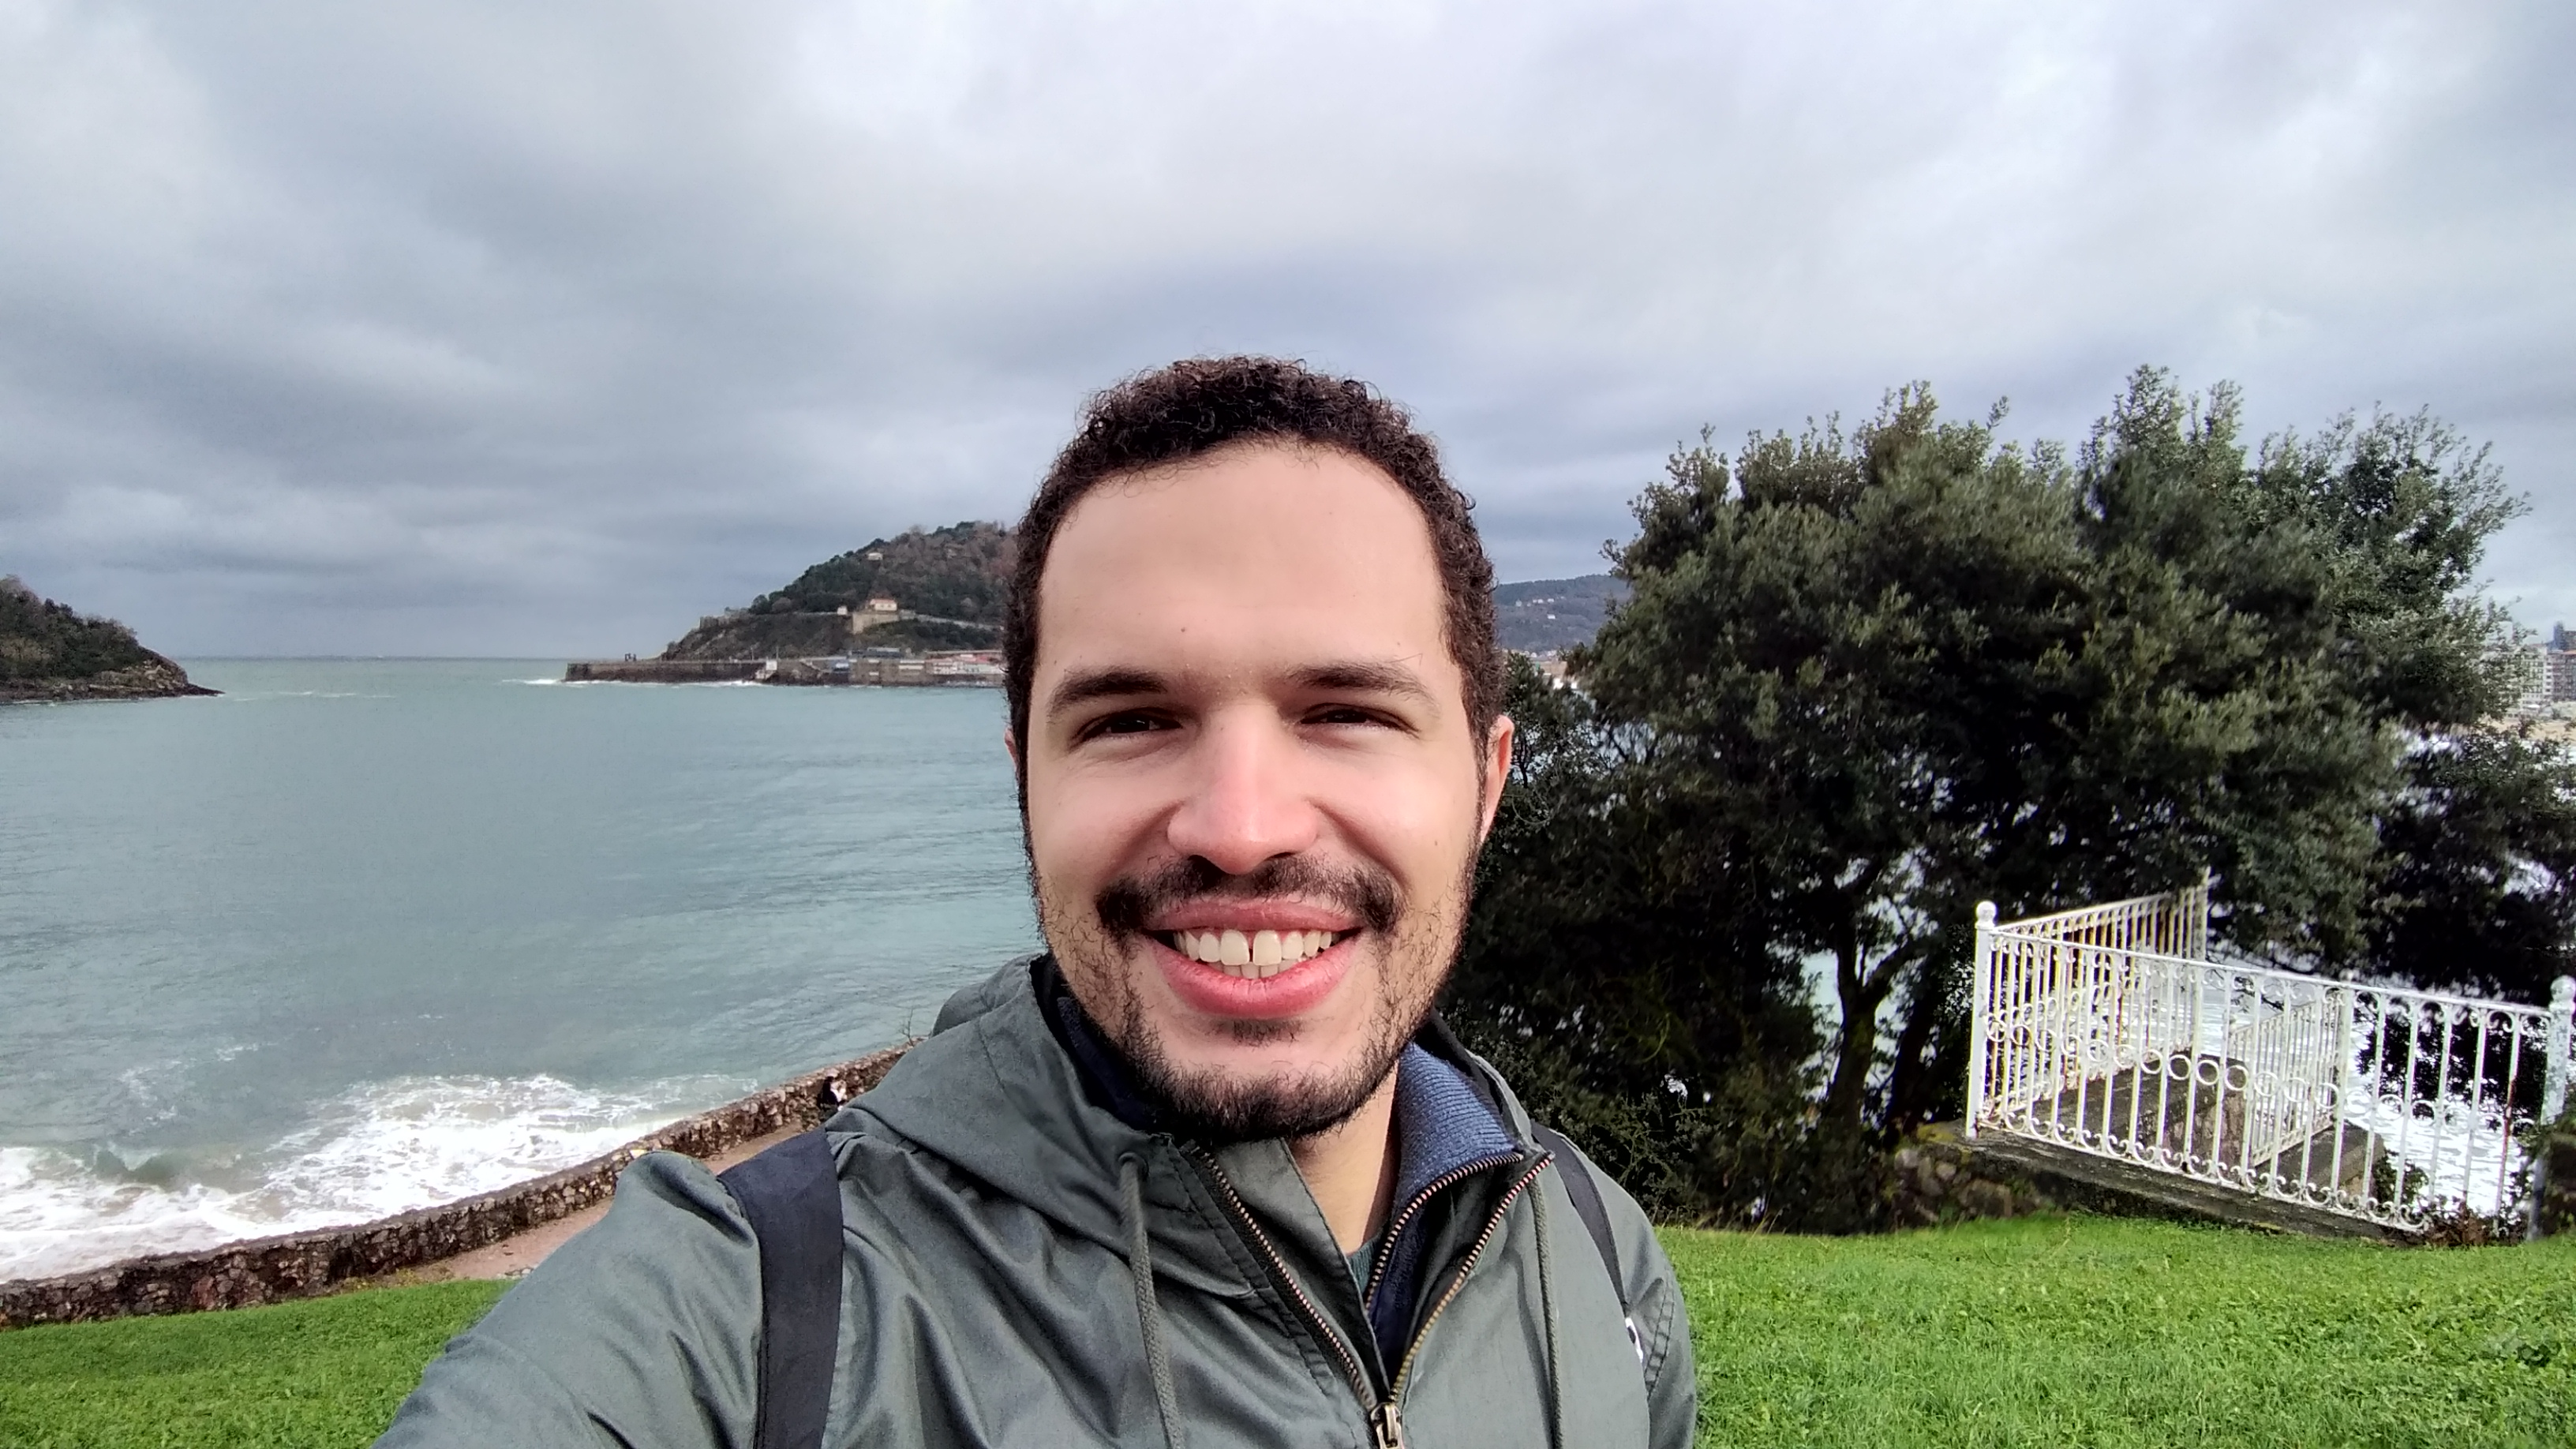
\includegraphics[trim=1000 200 1100 200,clip,scale=0.08]{diego.jpg}} % photo
    {\cvname{Diego Ferreira}
    
    \cvpersonalinfolinewithicon{height=4.5mm}{globe.png}{Brazil, Belo Horizonte} % address
    
    \cvpersonalinfolinewithicon{height=4.5mm}{phone.png}{+55 31 92000 2151} % phone number
    
    \cvpersonalinfolinewithicon{height=4.5mm}{envelope.png}{diegobragaferreira@gmail.com} % email address
    
    \cvpersonalinfolinewithicon{height=4.5mm}{envelope.png}{ferreira@fisica.ufmg.br} % email address
    
    \cvpersonalinfolinewithicon{height=4.5mm}{github.png}{/diegobragaferreira}
    
    \cvpersonalinfolinewithicon{height=4.5mm}{passport.png}{Brazilian, born in 15/Oct/1989}
    
    \cvpersonalinfolinewithicon{height=4.5mm}{comment.png}{
    I am a researcher scientist and PhD physics student at Federal University of Minas Gerais, Brazil, 
    and I work with various topics in Quantum Information and Condensed Matter Systems.
    I develop and apply Tensor Network techniques to theoretically 
    study the dynamics of Quantum many-body systems.
    I have experience in program development and simulations, using 
    C++, Matlab and Fortran, as well as in analytical solutions of selected models.
    My interest is advance the tensor network mathematical framework and solve 
    frontier science problems in Quantum Information and Condensed Matter Theory.}}

    
\cvsection{Area of research}

\cvitem{\cvdurationstyle{}}
    {\cvtitle{}
    Quantum Information, Condensed Matter and Statistical Physics.
    }    

\cvsection{Topics of Interest}

\cvitem{\cvdurationstyle{}}
    {\cvtitle{}
    \begin{itemize}[leftmargin=*]
    \item Many-body localization and thermalisation;
    \item Open dissipative dynamics;
    \item Tensor networks renormalization algorithms and numerical methods for time evolution of closed and open systems, for both 1D and 2D;
    \item Quantum phase transitions;
    \item Quantum correlations in systems of indistinguishable particles;
    \item The fermionic extended Hubbard model.
    \end{itemize}}

% education
\cvsection{Education}

% phd
\cvitem{\cvdurationstyle{2016 - Present}}
    {\cvtitle{Ph.D. in Physics}

    Quantum Information Group (Infoquant), Federal University of Minas Gerais (Brazil, Belo Horizonte)
    
        \begin{itemize}[leftmargin=*]
        \item \textit{Title:} Tensor Network Techniques applied in the study 
        of the Extended Hubbard Model and the Diamond Chain
        
        \item \textit{Advisor:} Prof. Reinaldo O. Vianna
        
        \item \textit{Co-advisor:} Prof. Fernando Iemini (UFF - Brazil, Rio de Janeiro)
        \end{itemize}}

% master
\cvitem{\cvdurationstyle{2014 - 2016}}
    {\cvtitle{M.Sc. in Physics}

    Quantum Information Group (Infoquant), Federal University of Minas Gerais (Brazil, Belo Horizonte)
    
    \begin{itemize}[leftmargin=*]
        \item \textit{Title:} Multipartite Entanglement in one-dimensional Tensor Networks in the MPS approximation
        
        \item \textit{Advisor:} Prof. Reinaldo O. Vianna
        
        \end{itemize}}

% bachelor
\cvitem{\cvdurationstyle{2010 - 2013}}
    {\cvtitle{B.Eng. in Physics with emphasis in Computational Physics }

    Federal University of Sao Joao del-Rei (Brazil, Minas Gerais)
    
    \begin{itemize}[leftmargin=*]
        \item \textit{Title:} Study of Effective Models for Quantum Cromodynamics: Equilibrium and Dynamics out of Equilibrium
        
    \item \textit{Advisor:} Prof. Ricardo L. S. Farias
    
    \end{itemize}}

% languages
\cvitem{\cvdurationstyle{}}
    {\cvtitle{Languages}
    
    \begin{itemize}[leftmargin=*]
        \item \textit{English:} Full professional proficiency
        
        \item \textit{Portuguese:} Native proficiency
        
        %\item \textit{Japanese:} Elementary proficiency
        \end{itemize}}

% professional experience
\cvsection{Professional Experience}

\cvitem{\cvdurationstyle{2016 - Present}}
    {\cvtitle{Ph.D. Researcher at UFMG (Brazil, Minas Gerais)}
    
    \begin{itemize}[leftmargin=*]
        \vspace{0.2cm}
        \item I doing my PhD working mainly on the subjects: (i) quantum phase transitions and analysis of the entanglement spectrum distribution of the two-body reduced density matrix in the Extended Hubbard Model, (ii) the presence of many-body localization in the diamond chain and its implications, and (iii) a purely dissipative Lindblad dynamics which can produced a geometrical frustrated 1D quantum system by competition of distinct dissipative channels in a non-equilibrium evolution. During this time I gained experience in developing various types of open and closed systems time evolution algorithms in C++, as well as a fast algorithm for calculating a fourth-order correlator in a fermionic system.
        \vspace{0.2cm}
        \item During my PhD I made a visit for a period of one month (2018) at the ICTP/Trieste in Italy, where I had the opportunity to attend a school which greatly added to my doctorate and allowed the collaboration that I have with Dr. Rosario Fazio and Prof. Dr. Fernando Iemini (postdoctoral fellow at the time). I also participate on a school for tensor network approaches to Quantum many-body systems, where I learned various topics on the state of the art of the tensor network theory, and I was able to develop more general and robust algorithms.
        \vspace{0.2cm}
        \item \textit{Achievements:} two manuscripts accepted in Physical Review A (impact factor 3.14) and Physical Review B (impact factor 4.036), one submitted in Physical Review B as first author (approved by referees and under small revisions), and other two under review in the peer review journals Physical Review A and Europhysics Letters (impact factor 1.957). Two poster presentations in international conferences. Two ongoing projects mentioned above, two of them as the first author: the first (on the Hubbard model) submitted, and the second (diamond chain) with preliminary results and a draft.
        \vspace{0.2cm}
        \item \textit{Skills:} Numerical modeling with Tensor Network formalism;
        analytical solving of many-body problems; experience in C++ and Matlab.
    \end{itemize}}

% mackenzie
\cvitem{\cvdurationstyle{2014 - 2016}}
    {\cvtitle{M.Sc. Researcher at UFMG (Brazil, Minas Gerais)}

    \begin{itemize}[leftmargin=*]
        \vspace{0.2cm}
        \item I worked in the understanding of the multipartite entanglement structure in the Ising Model, where I gained experience with tensor network methods (matrix product states and density matrix renormalization group in particular) in the study of many body systems, as well as the formal theory of quantum correlations.
        \vspace{0.2cm}
        \item \textit{Skills:} Numerical simulation of quantum 1D models.
    \end{itemize}}

\cvitem{\cvdurationstyle{2010 - 2013}}
    {\cvtitle{B.Eng. Researcher at UFSJ (Brazil, Minas Gerais)}
    
    \begin{itemize}[leftmargin=*]
        \vspace{0.2cm}
        \item I've worked with the bi-dimensional classical Ising Model, developing the Monte-Carlo algorithm for the system simulation and calculations of various thermodynamic quantities,studying the effect of bond dilution on these quantities. Later on, I’ve worked in a Quantum Field Theory laboratory studying analytical and numerical non-perturbative methods to solve a stochastic Langevin equation of motion for a scalar field (order parameter) in a effective QCD model.
        \vspace{0.2cm}
        \item \textit{Skills:} Numerical simulations using fortran.
    \end{itemize}}

    \newpage
% scientific production
\cvsection{Scientific Production}

\cvitem{\cvdurationstyle{Preprint}}
    {\cvtitle{Quantum correlations, entanglement spectrum and coherence of two-particle reduced density matrix in the Extended Hubbard Model}
    
    \vspace{0.2cm}
    \underline{Diego L. B. Ferreira}, Tiago O. Maciel, Reinaldo O. Vianna and Fernando Iemini.
    
    \vspace{0.2cm}
    arXiv:2111.00085 (2021)
    \textit{submitted to Physical Review B}}

\cvitem{\cvdurationstyle{Journal}}
    {\cvtitle{Determination of the critical exponents in dissipative phase transitions: coherent anomaly approach}
    
    \vspace{0.2cm}
    Jiasen Jin, Wen-Bin He, Fernando Iemini, \underline{Diego Ferreira}, Ying-Dan Wang, Stefano Chesi and Rosario Fazio.
    
    \vspace{0.2cm}
    Physical Review B, 104 (2021) 214301}
    
\cvitem{\cvdurationstyle{Preprint}}
    {\cvtitle{Quantum Statistical Complexity Measure as a Signalling of Correlation Transitions}
    
    \vspace{0.2cm}
    Andr\'e T. Ces\'ario, \underline{Diego L. B. Ferreira}, Tiago Debarba, Fernando Iemini, Thiago O. Maciel, Reinaldo O. Vianna.
    
    \vspace{0.2cm}
    arXiv:2002.01590 (2020)}
        
\cvitem{\cvdurationstyle{Preprint}}
    {\cvtitle{Probing Genuine Multipartite Entanglement in Large Systems}
    
    \vspace{0.2cm}
    Lucas B. Vieira, \underline{Diego L. Braga Ferreira}, Thiago O. Maciel and Reinaldo O. Vianna.
    
    \vspace{0.2cm}
    arXiv:1911.04649 (2019)}
        
\cvitem{\cvdurationstyle{Journal}}
    {\cvtitle{Completely positive maps for reduced states of indistinguishable particles}
    
    \vspace{0.2cm}
    Leonardo da Silva Souza, Tiago Debarba, \underline{Diego L. Braga Ferreira}, Fernando Iemini, and Reinaldo O. Vianna.
    
    \vspace{0.2cm}
    Physical Review A, 98 (2018) 052135}
    
% posters
\cvitem{\cvdurationstyle{Poster}}
    {\cvtitle{Tensor Network Techniques applied in the Extended
    Hubbard Model}
    
    \vspace{0.2cm}
    \underline{Diego L. Braga Ferreira}, Thiago O. Maciel, Fernando Iemini and Reinaldo O. Vianna.
    
    \vspace{0.2cm}
    Presented at ``Tensor Network based approaches to Quantum Many-Body Systems'', Donostia International Physics Center, Donostia-San Sebasti\'an, Spain (2019).}
    
\cvitem{\cvdurationstyle{Poster}}
    {\cvtitle{Tensor Network Techniques applied in the Extended
    Hubbard Model}
    
    \vspace{0.2cm}
    \underline{Diego L. Braga Ferreira}, Thiago O. Maciel, Fernando Iemini and Reinaldo O. Vianna.
    
    \vspace{0.2cm}
    Presented at ``Summer School on Collective Behaviour in Quantum Matter'', ICTP, Trieste, Italy (2018).}

% references
\cvsection{References}

\cvitem{\cvdurationstyle{}}
    {\cvtitle{Prof. Reinaldo Oliveira Vianna}
    
    \emph{Infoquant} Quantum Information Group, Federal University of Minas Gerais (Brazil, Minas Gerais)
    
    \vspace{0.2cm}
    Email: reinaldo@fisica.ufmg.br}

\cvitem{\cvdurationstyle{}}
    {\cvtitle{Prof. Fernando Iemini}
    
    Physics Institute, Fluminense Federal University (Brazil, Niter\'oi)
    
    \vspace{0.2cm}
    Email: fiemini@mail.if.uff.br}

\cvitem{\cvdurationstyle{}}
    {\cvtitle{Dr. Thiago O. Maciel}
    
    GIQSUL, Federal University of Santa Catarina (Brazil, Santa Catarina)
    
    \vspace{0.2cm}
    Email: maciel@gmail.com}

\end{document}
